% !TEX program = xelatex
% sglang-rbln design review  —  SqueezeBits 2nd assessment
% Compile with XeLaTeX (Overleaf: Menu -> Compiler -> XeLaTeX; latexmkrc already sets this).
\documentclass[aspectratio=169,11pt,dvipsnames]{beamer}
\usetheme{metropolis}

\usepackage{fontspec}
\usepackage{kotex}                 % Korean (XeLaTeX). Remove if you go English-only.
\usepackage{amssymb,amsmath}
\usepackage{booktabs}
\usepackage{tikz}
\usetikzlibrary{arrows.meta,positioning,calc,fit,backgrounds}

% ---- palette (matches the brick-red the PPT drafts used) ----
\definecolor{brick}{HTML}{C03221}
\definecolor{ink}{HTML}{1A1A1A}
\definecolor{paper}{HTML}{FFFDFB}
\definecolor{soft}{HTML}{ECE7E3}
\definecolor{softtxt}{HTML}{5A5550}

\setbeamercolor{normal text}{fg=ink,bg=paper}
\setbeamercolor{alerted text}{fg=brick}
\setbeamercolor{frametitle}{fg=ink,bg=paper}
\setbeamercolor{progress bar}{fg=brick}
\setbeamercolor{title separator}{fg=brick}
\metroset{block=fill,sectionpage=none,numbering=fraction,progressbar=frametitle}

% red rule under every frame title
\setbeamertemplate{frametitle}{%
  \nointerlineskip
  \begin{beamercolorbox}[wd=\paperwidth,sep=0.85ex,leftskip=1.4ex]{frametitle}%
    \usebeamerfont{frametitle}\strut\insertframetitle\strut\par
  \end{beamercolorbox}%
  {\color{brick}\rule{\paperwidth}{1pt}}\par\vspace*{0.4ex}%
}

\setbeamertemplate{itemize item}{\textcolor{brick}{\textbf{--}}}
\setbeamertemplate{itemize subitem}{\textcolor{softtxt}{$\cdot$}}

% section header used inside frames (the style used in the PPT drafts)
\newcommand{\hd}[1]{{\color{brick}\bfseries #1}\par\smallskip}
% inline residual symbols
\newcommand{\R}{\ensuremath{R}}
\newcommand{\Sfull}{\ensuremath{S}}

\setlength{\parskip}{2pt}


\title{sglang-rbln 설계 리뷰}
\subtitle{vllm-rbln에서 유추한 RBLN 소프트웨어 스택 특성 기반 설계 / 구현}
\author{손성욱 \; (Sungwook Son)}
\date{2026.09.04 \quad\textbar\quad SqueezeBits Efficiency Part — 2nd assessment}

\begin{document}

\maketitle

\begin{frame}{발표 순서}
  \small
  \begin{columns}[T]
    \begin{column}{0.5\textwidth}
      \begin{itemize}\setlength\itemsep{4pt}
        \item[Q1] Strict AOT — 재사용 vs 재설계
        \item[Q2] 고정 shape 버킷 / warm-up의 한계
        \item[Q3] Prefix caching과 prefill 버킷 설계
        \item[Q4] 포팅 계획이 틀어진 사례
        \item[Q5] 컴파일 스펙트럼별 강제사항
      \end{itemize}
    \end{column}
    \begin{column}{0.5\textwidth}
      \begin{itemize}\setlength\itemsep{4pt}
        \item[Q6] RadixAttention vs PagedAttention
        \item[Q7] 스케줄러 차이 · host 병목
        \item[Q8] RadixAttention의 RBLN 포팅 경계
        \item[Q9] AOT에서 speculative decoding
        \item[Q10] TPOT P99 악화 분석
      \end{itemize}
    \end{column}
  \end{columns}
\end{frame}

\begin{frame}{전제 — vllm-rbln에서 읽어낸 RBLN 스택}
  \begin{itemize}\setlength\itemsep{5pt}
    \item \textbf{완전 AOT} — 런타임 컴파일 / eager fallback 없음; 미준비 shape은 실행 불가.
    \item \textbf{두 경로} — optimum-rbln \texttt{.rbln} 아티팩트 \,/\, \texttt{torch.compile(dynamic=False)} + rebel backend.
    \item \textbf{Prefill 단독}(batch $=1$); \textbf{decode batch만 버킷팅}; seq len은 고정 \texttt{max\_model\_len} 그래프.
    \item \textbf{KV block $=$ attention partition} (1--4K tok) $\Rightarrow$ sub-block prefix caching; hit 시 KV \emph{복사}(동기).
    \item \textbf{TP는 그래프에 컴파일}; \textbf{overlap scheduler 없음}.
  \end{itemize}
  \begin{alertblock}{한 줄}
    RBLN은 strict-AOT — 미준비 shape에 런타임 탈출구가 없다. 나머지 설계는 여기서 파생.
  \end{alertblock}
\end{frame}


% ============================ Q1 ============================
\begin{frame}{Q1 — Strict AOT: 재사용 vs 재설계}
  \footnotesize
  \hd{Framing}
  Gaudi has a runtime escape hatch (JIT recompile on a shape miss); RBLN does not — an
  uncompiled shape cannot run. Reference experience: vLLM-on-Gaudi, one step less strict.

  \hd{Carries over — disciplines, not code}
  \begin{itemize}
    \item Shape normalization at the scheduler boundary (bucket $\to$ pad $\to$ mask).
    \item Separate prefill / decode graph families.
    \item Sampling, penalties, grammar, detokenize kept \emph{off} the model graph.
    \item Host-side KV / paging / radix bookkeeping — SGLang's \texttt{RadixCache} is already host Python.
    \item Offline compile + artifact cache + CI precompile; shape telemetry $\to$ offline re-bucketing.
  \end{itemize}

  \hd{Must be redesigned}
  \begin{itemize}
    \item Forward path (eager torch + CUDA graphs / FlashInfer / Triton $\to$ precompiled runtime).
    \item Mixed prefill+decode batching (vllm-rbln forbids it: prefill exclusive, batch 1).
    \item RadixAttention's variable extend length; jump-forward / retract / adaptive trees.
    \item Speculative decoding; per-op NCCL TP; the overlap scheduler.
  \end{itemize}
\end{frame}

\begin{frame}{Q1 — meta-lesson}
  \begin{alertblock}{Invariant, designed in from commit 1}
    The scheduler emits \emph{only} shapes compiled offline.
  \end{alertblock}
  \begin{itemize}
    \item A clamp layer maps any (batch, chunk, block-count) to the nearest warmed bucket.
    \item A bounded, loudly-metered fallback-compile path — \emph{never} on the serving hot path.
    \item On Gaudi I could lean on recompile-on-miss during bring-up; it bit back later as
          mid-serving JIT stalls. RBLN forces the invariant early.
  \end{itemize}
\end{frame}

\begin{frame}{Q2 — 고정 shape 버킷 / warm-up의 한계}
  \hd{Why bucket at all}
  NPUs only run compiled fixed-shape graphs; a serving-path recompile is unacceptable
  $\Rightarrow$ every shape is compiled at warm-up.

  \hd{Gaudi limits (pre-chunked-prefill, vLLM V0)}
  \begin{itemize}
    \item Prompt bucket $=$ (bs $\times$ seq\_len) $\Rightarrow$ count scales with \texttt{max\_model\_len}
          — 24 prompt $+$ 48 decode in the docs; 100s--1000s for long context.
    \item Warm-up is a deploy cost: a $\sim$1M-token config OOM'd; when it fit, 24h$+$ to compile.
    \item An unbucketed request $\Rightarrow$ synchronous recompile that stalls the \emph{whole} engine.
  \end{itemize}

  \hd{Mitigations}
  \begin{itemize}
    \item Exponential / padding-aware bucketing (\texttt{pad\_max}, \texttt{pad\_percent}) — 1000s $\to$ $\sim$13.
    \item Graph caching — compile once, save to host, reuse across restarts / pods.
    \item Chunked prefill (V1): bucket $=$ (bs $\times$ query $\times$ num\_blocks), query capped at chunk size
          $\Rightarrow$ prompt-bucket count \emph{decouples} from \texttt{max\_model\_len}
          ($\sim$36 prompt, $\sim$100$\times$ the context).
  \end{itemize}
\end{frame}

\begin{frame}{Q3 — Prefix caching과 prefill 버킷 설계}
  \hd{The effect}
  \begin{itemize}
    \item Without caching, buckets are sized to the full prompt length.
    \item With a hit, tokens actually computed $= R = (\text{prompt}) - (\text{cached prefix})$;
          $R$ varies per request, usually small.
    \item Pick the bucket from $R$, not the prompt — a prompt-sized graph pads away the benefit.
  \end{itemize}
  \hd{Approach}
  \begin{itemize}
    \item Look up cache $\to$ compute $R$ $\to$ smallest compiled bucket $\ge R$.
    \item One chunk-sized prefill graph $+$ a few tail buckets; long $R$ repeats the chunk.
    \item Bucket sizes from the real post-cache $R$ distribution, recompiled offline.
    \item vllm-rbln: one prefill graph at chunk size; sub-block reuse; matched KV copied before the forward.
  \end{itemize}
\end{frame}

\begin{frame}{Q3 — how prefix caching moves the workload}
  \vspace{1.2em}
  \begin{center}\resizebox{\textwidth}{!}{% S = cached prefix + residual R  ->  bucket is chosen from R
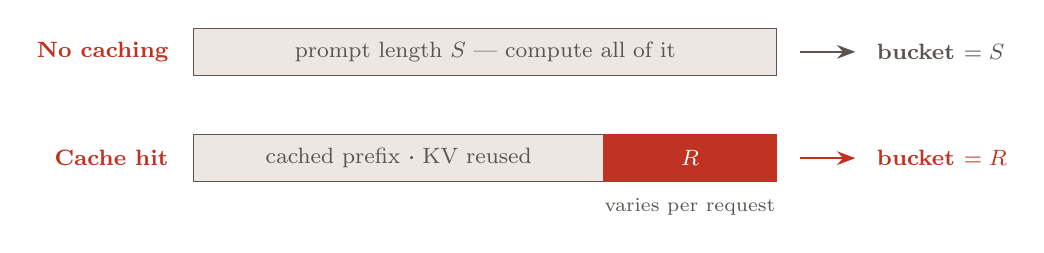
\begin{tikzpicture}[font=\footnotesize, x=1cm, y=1cm]
  % Row 1: no caching
  \node[anchor=east, brick, font=\footnotesize\bfseries] at (-0.2,1.35) {No caching};
  \filldraw[fill=soft, draw=softtxt] (0,1.05) rectangle (7.4,1.65);
  \node[softtxt] at (3.7,1.35) {prompt length $S$ — compute all of it};
  \draw[-{Stealth}, softtxt, thick] (7.7,1.35) -- (8.4,1.35);
  \node[anchor=west, softtxt, font=\footnotesize\bfseries] at (8.55,1.35) {bucket $=S$};

  % Row 2: cache hit
  \node[anchor=east, brick, font=\footnotesize\bfseries] at (-0.2,0.0) {Cache hit};
  \filldraw[fill=soft, draw=softtxt] (0,-0.3) rectangle (5.2,0.3);
  \node[softtxt] at (2.6,0.0) {cached prefix · KV reused};
  \filldraw[fill=brick, draw=brick] (5.2,-0.3) rectangle (7.4,0.3);
  \node[white, font=\footnotesize\bfseries] at (6.3,0.0) {$R$};
  \node[softtxt, font=\scriptsize] at (6.3,-0.62) {varies per request};
  \draw[-{Stealth}, brick, thick] (7.7,0.0) -- (8.4,0.0);
  \node[anchor=west, brick, font=\footnotesize\bfseries] at (8.55,0.0) {bucket $=R$};
\end{tikzpicture}
}\end{center}
  \vspace{1.6em}
  \footnotesize A short $R$ still attends over the \emph{full} cached context
  $\Rightarrow$ the graph needs a small query bucket \textbf{and} a bounded pointer to the
  cached KV (block table $+$ seq-lens), not one large shape.
\end{frame}

% ============================ Q4 ============================
\begin{frame}{Q4 — 포팅 계획이 틀어진 사례와 교훈}
  \footnotesize
  \hd{Wrong assumption}
  Ported Qwen2.5/3-VL to Gaudi. LLM already ran; ``the vision encoder is just a transformer''
  $\Rightarrow$ scoped it as wrap-the-whole-encoder-in-one-graph.

  \hd{What broke}
  Vision-tower sequence length $=$ total patch count $= \sum_{\text{images}} t\cdot h\cdot w$
  — varies with image count, resolution, aspect ratio $\Rightarrow$ \texttt{cu\_seqlens},
  block-diagonal mask shape, window partitioning all data-dependent $\Rightarrow$ one static
  graph impossible. Team pushed on a pure graph for weeks.

  \hd{Resolved in phases}
  \begin{itemize}
    \item per-image loop $\to$ patch-count bucketing (pad hidden states / RoPE / \texttt{cu\_seqlens}, strip after)
    \item split the tower: \textbf{pre\_attn (dynamic) / static core (compiled) / post\_attn (dynamic)}
    \item operator-declared warm-up (resolution $\times$ item-count, incl. ranges for the cache interaction)
  \end{itemize}
  Never fully static — mask still CPU-fallbacks for long sequences; long-seq attention still tiles.

  \hd{Lesson $\to$ sglang-rbln}
  Don't eliminate dynamism, \emph{relocate} it: largest possible static core, thin dynamic shell on the host.
  $\Rightarrow$ encoder+projector as a separate compiled unit; pre/static/post as the default structure;
  bucket by patch count; warm-up manifest; miss-guard with a bounded loud fallback.
\end{frame}

% ============================ Q5 ============================
\begin{frame}{Q5 — 컴파일 스펙트럼별 강제사항}
  \footnotesize
  \hd{Reframe}
  Not about ``compilation'' — about what the stack may assume about shapes, and what a miss costs.

  \begin{itemize}
    \item \textbf{Eager} — total shape freedom; host is the bottleneck (launch per op).
          Design: C++ hot path, overlap, minimal per-step Python.
    \item \textbf{JIT + cache} — first hit compiles; soft bucketing (a miss is slow, not fatal);
          versioned cache; SLO guard. Tolerates new shapes.
    \item \textbf{Graph capture / replay} — fixed shapes \emph{and} fixed addresses; pre-alloc KV/IO,
          copy-in/out; no data-dependent control flow inside the region.
    \item \textbf{Strict AOT} — shape set frozen at build; compiler version $=$ deploy contract;
          uncompiled shape cannot run $\Rightarrow$ scheduler must guarantee legal shapes;
          every dynamic path $=$ fixed-shape compute $+$ host post-processing.
  \end{itemize}

  \hd{My environments}
  \begin{itemize}
    \item Gaudi $=$ capture/replay $+$ JIT-recompile fallback. Precompile the covering set — a miss stalls the whole engine.
    \item Battlemage $=$ eager, \emph{forced} by oneCCL/SYCL not composing (no multi-card). Single-card, host-path optimized.
  \end{itemize}
\end{frame}

\begin{frame}{Q5 — the spectrum}
  \vspace{1.5em}
  \begin{center}% compile spectrum: constraints tighten left -> right
\begin{tikzpicture}[font=\scriptsize, x=1cm, y=1cm]
  \draw[-{Stealth}, softtxt, very thick] (0,0) -- (13.2,0);
  \foreach \x/\name in {0.6/Eager, 4.6/{JIT + cache}, 8.2/{Graph capture / replay}, 11.8/{Strict AOT}}{
    \fill[brick] (\x,0) circle (2.2pt);
    \node[anchor=south, brick, font=\scriptsize\bfseries] at (\x,0.18) {\name};
  }
  \node[anchor=north, softtxt, text width=3.2cm, align=center] at (0.6,-0.25)
    {shape 완전 자유\\host가 병목};
  \node[anchor=north, softtxt, text width=3.4cm, align=center] at (4.6,-0.25)
    {첫 히트 컴파일\\soft 버킷팅 · 미스=느림};
  \node[anchor=north, softtxt, text width=3.6cm, align=center] at (8.2,-0.25)
    {고정 shape \emph{및} 고정 주소\\region 내 제어흐름 금지};
  \node[anchor=north, softtxt, text width=3.4cm, align=center] at (11.8,-0.25)
    {build에 shape 확정\\미스 = 실행 불가};
  \node[anchor=west, brick, font=\scriptsize] at (0,-1.9)
    {Gaudi $\approx$ capture/replay $+$ JIT fallback \quad\textbar\quad Battlemage $\approx$ eager (toolchain-forced) \quad\textbar\quad RBLN $=$ strict AOT};
\end{tikzpicture}
\end{center}
  \vspace{1em}
  \small For sglang-rbln: RBLN sits at strict-AOT with no fallback $\Rightarrow$ ``keep shapes legal''
  moves entirely into the scheduler $+$ build pipeline. Gaudi's discipline, safety net removed.
\end{frame}

\begin{frame}{Q6 — RadixAttention vs PagedAttention}
  \hd{Different layers, not competitors}
  \begin{itemize}
    \item \textbf{PagedAttention} $=$ a KV-cache \emph{memory allocator} (blocks $+$ block table).
    \item \textbf{RadixAttention} $=$ a \emph{reuse $+$ eviction policy} (prefix tree $+$ LRU).
    \item You need both. Real comparison: RadixAttention vs vLLM's hash-based prefix caching.
  \end{itemize}
  \hd{AOT burden — all from ``block $=$ fixed attention partition (1--4K)''}
  \begin{itemize}
    \item Granularity fights the kernel $\Rightarrow$ a separate sub-block caching layer.
    \item A prefix hit is a \emph{physical KV copy} (sync, all layers, before the forward).
    \item Tree bookkeeping is host work on the critical path; eviction fenced to step boundaries.
    \item Variable match length $\Rightarrow$ variable prefill shape $\Rightarrow$ forced to a fixed chunk.
    \item HiCache (L1/L2/L3): an L2/L3 hit stalls for a promotion; a slow fetch $\to$ recompute.
  \end{itemize}
  \begin{alertblock}{Mitigation}
    Pin the reuse granularity to a sub-block $=$ the prefill chunk size (what vllm-rbln did).
  \end{alertblock}
\end{frame}

% ============================ Q7 ============================
\begin{frame}{Q7 — SGLang vs vLLM 스케줄러 · host 병목}
  \footnotesize
  \hd{How SGLang differs}
  \begin{itemize}
    \item \textbf{Overlap scheduler} — build the next batch on CPU while the current runs on device. The defining feature.
    \item Radix / cache-aware admission (longest-prefix-match first); FSM $+$ jump-forward integrated into scheduling.
    \item vLLM v1: separate EngineCore process, chunked prefill by default, token-budget scheduling.
  \end{itemize}

  \hd{Importance for RBLN — the top TPOT lever}
  \begin{itemize}
    \item Decode device step is short and fixed $\Rightarrow$ host fraction (batch build, match, block-table,
          H2D, per-step mask, sampling, detok) dominates.
    \item host $\ge$ device $\Rightarrow$ host-bound $\Rightarrow$ TPOT set by the scheduler loop, not the chip.
    \item AOT removes the graph-capture escape hatch $\Rightarrow$ overlap is close to mandatory.
    \item vllm-rbln evidence: pinned \texttt{\_to\_list}, per-step host masks, Python-loop KV copies, async scheduling disabled.
    \item Porting SGLang's overlap scheduler $=$ \textbf{greenfield} (nothing to replace).
    \item Caveat: TTFT / long prefill is device-bound — this is a decode / TPOT lever.
  \end{itemize}

  \begin{block}{Judgment basis}
    Measure device-exec vs wall step time at target batch. host critical path $>$ device exec $\Rightarrow$ scheduler is the top lever.
    \emph{[insert your own host-bottleneck example: measurement, \% host, what you changed.]}
  \end{block}
\end{frame}

% ============================ Q8 ============================
\begin{frame}{Q8 — RadixAttention의 RBLN 포팅 경계}
  \small
  The radix tree is \emph{entirely} host. The device does fixed-shape matmuls $+$ KV scatter
  $+$ one host-scheduled block copy.
  \vspace{0.6em}
  \begin{center}% host / device boundary for RadixAttention on RBLN
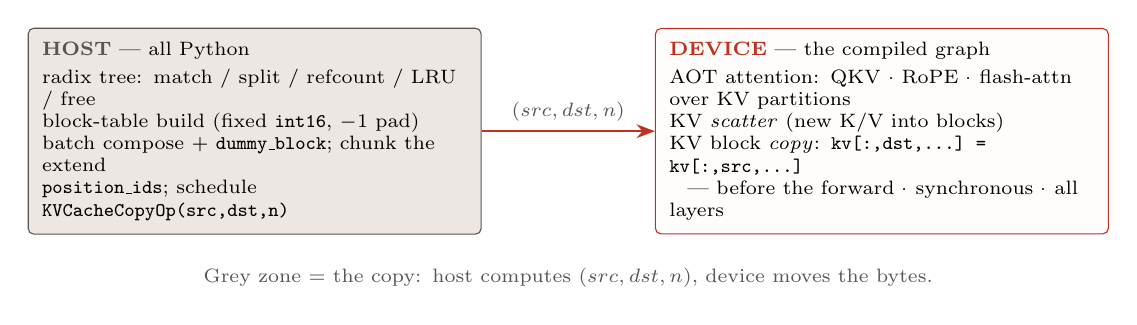
\begin{tikzpicture}[font=\scriptsize, node distance=4mm]
  \tikzset{
    hostbox/.style={draw=softtxt, fill=soft, rounded corners=2pt, text width=5.4cm, inner sep=5pt, align=left},
    devbox/.style ={draw=brick,   fill=paper, rounded corners=2pt, text width=5.4cm, inner sep=5pt, align=left},
  }
  \node[hostbox] (h) {
    \textbf{\textcolor{softtxt}{HOST}} — all Python\\[2pt]
    radix tree: match / split / refcount / LRU / free\\
    block-table build (fixed \texttt{int16}, $-1$ pad)\\
    batch compose $+$ \texttt{dummy\_block}; chunk the extend\\
    \texttt{position\_ids}; schedule \texttt{KVCacheCopyOp(src,dst,n)}
  };
  \node[devbox, right=2.2cm of h] (d) {
    \textbf{\textcolor{brick}{DEVICE}} — the compiled graph\\[2pt]
    AOT attention: QKV · RoPE · flash-attn over KV partitions\\
    KV \emph{scatter} (new K/V into blocks)\\
    KV block \emph{copy}: \texttt{kv[:,dst,\dots] = kv[:,src,\dots]}\\
    \hphantom{x}\;— before the forward · synchronous · all layers
  };
  \draw[-{Stealth}, brick, thick] (h.east) -- node[above, midway, softtxt]{$(src,dst,n)$} (d.west);
  \node[below=3mm of $(h.south)!0.5!(d.south)$, softtxt, text width=11.5cm, align=center]
    {Grey zone $=$ the copy: host computes $(src,dst,n)$, device moves the bytes.};
\end{tikzpicture}
\end{center}
\end{frame}

\begin{frame}{Q8 — porting order}
  \small
  \begin{enumerate}\itemsep2pt
    \item KV pool layout \texttt{[2, num\_blocks, H, 1, block\_size, D]}; \texttt{block\_size} $=$ partition.
    \item Fixed-shape prefill / decode graph interfaces (one chunk size; batch-size buckets).
    \item RBLN \texttt{AttentionBackend} — translate SGLang forward metadata into the fixed tensors.
    \item Compile the covering set $+$ artifact cache (keyed on model / dtype / TP / bucket-hash / compiler).
    \item Host radix layer — align matched prefixes to sub-block $=$ chunk size.
    \item KV write / reuse — scatter for new K/V; schedule a copy op for a partial hit.
    \item Absolute-position RoPE; scheduler guard (only compiled shapes); step-fenced eviction.
    \item TP (collectives in-graph); correctness $+$ boundary validation; shape telemetry.
  \end{enumerate}
\end{frame}

\begin{frame}{Q9 — AOT에서 speculative decoding (EAGLE)}
  \hd{Setup} A small draft head predicts $k$ tokens AR from the target's hidden states;
  the target verifies in one forward; the accepted prefix is committed.
  \hd{AOT problems}
  \begin{itemize}
    \item Variable accept length $0..k$ $\Rightarrow$ always run the fixed verify graph, select on host;
          write KV for all $k$, advance \texttt{seq\_len} by accepted count.
    \item Tree mask $\Rightarrow$ a compiled attention variant, fixed max size/depth.
    \item Draft AR loop $=$ $k$ tiny sequential calls $\Rightarrow$ unroll into one graph.
    \item Hidden-state feedback plumbing; separate draft KV; $[k,\text{vocab}]$ D2H $+$ host rejection sampling.
  \end{itemize}
  \hd{What vllm-rbln shipped}
  EAGLE/EAGLE3 self-draft $+$ Medusa \emph{only}; no parallel drafting; \textbf{chain, not tree};
  $k{-}1$ steps $=$ a Python loop of separate compiled calls.
  \begin{alertblock}{Universal AOT pattern}
    Always compute the maximum, select on the host.
  \end{alertblock}
\end{frame}

\begin{frame}{Q10 — TTFT OK, TPOT P99 나쁨}
  \hd{Read the symptom}
  TTFT OK $\Rightarrow$ prefill / TP / plumbing fine. TPOT-\emph{P99} bad (not the mean)
  $\Rightarrow$ intermittent decode-loop stalls.
  \hd{Diagnosis, in order}
  \begin{enumerate}\setlength\itemsep{1pt}
    \item Span-instrument one decode step; per-step histograms.
    \item Queueing vs service (low load vs target QPS).
    \item Prefill interference; bucket / graph-switch cost.
    \item Device-exec variance at a \emph{fixed} bucket ($\Rightarrow$ compiler / runtime).
    \item Host critical path — GC, detok, non-overlapped copies ($\Rightarrow$ serving).
    \item Copy \& sync; collectives; eviction / prefix-hit KV copies.
  \end{enumerate}
\end{frame}

\begin{frame}{Q10 — attribution \& method}
  \hd{Team attribution}
  \begin{itemize}
    \item \textbf{serving} — queue / batching / bucket policy / overlap / host structures.
    \item \textbf{compiler} — per-op time at fixed shape, kernel schedule, graph-switch
          (signal: device P99 $\gg$ P50, same bucket).
    \item \textbf{runtime} — D2H mechanism, graph load/switch, collectives, \texttt{\_copy\_kv\_cache}.
  \end{itemize}
  \hd{Method}
  Load-sweep fixed lengths $\to$ realistic mix $\to$ stack P50/P95/P99 components $\to$
  the one whose P99/P50 ratio explodes is the culprit $\to$ bisect by feature toggles.
  \vspace{2pt}
  \footnotesize\emph{[insert your own latency triage: the breakdown, the culprit, the fix, which team.]}
\end{frame}


% ============================ CLOSE ============================
\begin{frame}{합류 시 첫 마일스톤 · 리스크}
  \small
  \hd{Milestones}
  \begin{itemize}
    \item \textbf{M0} — 1 model · TP1 · greedy · prefix cache off: compile $\to$ artifact $\to$ load $\to$ fixed-shape forward, end to end.
    \item \textbf{M1} — RBLN \texttt{AttentionBackend} $+$ fixed-chunk prefill $+$ decode-batch bucketing.
    \item \textbf{M2} — host radix $+$ sub-block prefix caching $+$ KV copy path.
    \item \textbf{M3} — overlap scheduler (greenfield) — the TPOT lever.
  \end{itemize}
  \hd{Risks / guards}
  \begin{itemize}
    \item Compiler rejects varlen attention · warm-up time (long context) · KV-copy sync cost · spec-decode scope.
    \item Scheduler shape-clamp $+$ bounded, loud fallback — never on the serving hot path.
    \item Shape telemetry $\to$ offline recompile.
  \end{itemize}
  \begin{alertblock}{One sentence}
    RBLN already keeps the Python scheduler thin and pushes variability into the compiled binary.
    sglang-rbln starts from that posture and adds the overlap scheduler.
  \end{alertblock}
\end{frame}

\begin{frame}[standout]
  감사합니다 \\[0.4em] Q \& A
\end{frame}


\end{document}
